\begin{comment}
\section{Osservabili stellari/demo beamer}
\begin{frame}<1>[label=noinside]{Modello stellare}{Come indagare la fisica interna a una stella?}
\onslide<1->\begin{block}{Osservabili stellari:}
$L$, $M$, $R$, $T_e$, $(\frac{Z}{X})_{ph}$, $g_{ph}$.
\end{block}
\onslide<1->\begin{block}{Informazioni sulla struttura interna?} Condizione di equilibrio idrostatico
\end{block}
%Teorema Vogt-Russel: $X_i(r)$, $M$ \pause equilibrio (idrostatico/termico) determinano struttura stellare .
%\pause
\onslide<1->\begin{block}{Modello stellare: diagramma di \hr{}.}
\end{block}
\onslide<2->\begin{block}{Descrizione fisica interno stellare: parametri aggiuntivi}
Convezione, diffusione e sedimentazione elementi pesanti, equazione di stato, opacit\'a
\end{block}
\onslide<2->\begin{block}{Astrosismologia}
Restringo spazio parametri sistemi stellari lontani
\end{block}
\end{frame}
{ % all template changes are local to this group.
    \setbeamertemplate{navigation symbols}{}
    \begin{frame}[plain]{Diagramma di \hr{}}
        \begin{tikzpicture}[remember picture,overlay]
            \node[at=(current page.center)] {
                %\includegraphics[width=\paperwidth]{yourimage}
            };
        \end{tikzpicture}
     \end{frame}
}
\againframe<2>{noinside}
\begin{frame}{Pulsazioni stellari}{Modi Normali}
\begin{columns}
\begin{column}{0.5\textwidth}  %%<--- here
    \begin{center}
     %\includegraphics[width=0.5\textwidth]{image1}
     \end{center}
\end{column}
\begin{column}{0.5\textwidth}
\onslide<1-> \begin{block}{Stelle pulsanti}
Onde stazionarie: Pulsazione radiale/non radiale: .
\onslide<2-> meccanismo di eccitazione: solar-like pulsator, Cefeidi.
\onslide<3-> Modo fondamentale $\Pi\approx\tau_{dyn}=\sqrt{\frac{R^3}{GM}}\propto\overline{\rho}\expy{-\frac{1}{2}}$.
\onslide<4-> Modi di oscillazione\onslide<5-> - informazioni sull'interno stellare
\onslide<5-> Elio-sismologia: Modi $\Leftrightarrow$ Modelli solari
\onslide<5-> Astero-sismologia: Modi $\Leftrightarrow$ Spazio parametri modello stellare
\end{block}
\end{column}
\end{columns}
\end{frame}

\end{comment}

\section{Osservabili solari}

\begin{frame}{Dati osservativi}

\begin{block}{Et\'a, luminosit\'a, raggio solari}
\begin{tabular}{l|c}
\hline
$\agesun{}$&\SI[separate-uncertainty=true]{4.57\pm0.02e9}{\year}\\
\hline
$\rsun{}$&\SI{695658+-140}{\kilo\meter}\\
\hline
$G\msun$&\num{132712440018+-8}\SI{e9}{\cubic\meter\per\square\second}\\
\hline
$\lsun{}$&\SI{3.8275+-0.0014e33}{\erg\per\second}\\
\hline
\end{tabular}
%\caption[Osservabili solari principali.]{Osservabili solari principali. \cite{haberreiter2008solving}.}
\label{tab:sunO}
\end{block}

\begin{block}{Simmetria sferica}
Deviazioni da forma sferica trascurabili (campi magnetici, rotazione)
\end{block}

\end{frame}

\begin{frame}{Dati osservativi}

\begin{block}{Composizione chimica}
\begin{itemize}
\item Righe di assorbimento: attuale (non $Y_{ph}$)
\item Meteoriti CI: primordiale (refrattari)
\end{itemize}

\begin{table}[]

\pgfplotstabletypeset[
every head row/.style={
 before row={\toprule &\multicolumn{4}{c|}{Attuale}
 %&\multicolumn{4}{c|}{Primordiale}
 \\\midrule},
 every last row/.style={after row=\bottomrule},
 after row={\midrule}
},
every nth row={2}{before row=\midrule},every last row/.style={after row=\bottomrule},
every first column/.style={column type/.add={|}{}},
every last column/.style={column type/.add={}{|}},
columns/x/.style = {column type/.add={|}{}},
columns/xi/.style = {column type/.add={|}{}},
display columns/0/.style={column name={}},
display columns/1/.style={column name={$X$}},
display columns/2/.style={column name={$Y$}},
display columns/3/.style={column name={$Z$}},
display columns/4/.style={column name={$\frac{Z}{X}$}},
%display columns/5/.style={column name={$X$}},
%display columns/6/.style={column name={$Y$}},
%display columns/7/.style={column name={$Z$}},
%display columns/8/.style={column name={$\frac{Z}{X}$}},
create on use/authors/.style={create col/set list={
%Anders \& Grevesse (1989),Grevesse \& Noels (1993),
Grevesse et al. (1998),Lodders (2003),Asplund et al. (2005),Lodders et al. (2009),\cite{asplund2009chemical},\cite{caffau2011solar}}},
columns/authors/.style={string type},
columns={authors,x, y, z, zx
%,xi,yi,zi, zxi
},
/pgf/number format/precision=4
     ]{asplund.txt} %%%
\captionof{table}{Metallicit\'a attuale determinata da varii autori.}\label{tab:Zhistory}
\end{table}

\end{block}

\end{frame}


\section{Strutture autogravitanti in equilibrio}

\begin{frame}{Distribuzione di massa - Conservazione di massa e momento}

\begin{block}{Massa}

%\begin{align}
%&dm=4\pi r^2\rho \,dr-4\pi r^2\rho v\,dt\label{eq:massvar}\\
%\end{align}

\begin{equation}
\PDy{t}{\rho}+\nabla\cdot(\rho\vec{v})=0\label{eq:continuityeq}
\end{equation}

\begin{equation}
dm=4\pi r^2\rho \,dr\label{eq:massaguscio}
\end{equation}

\end{block}

\begin{block}{Momento}
\begin{align}
&\rho\TDy{t}{\vec{v}}=-\nabla P+\rho\vec{f}\label{eq:motion}\\
&\vec{g}=-\PDy{r}{\Phi}=-\frac{Gm(r)}{r^2}\hat{r}
\end{align}
\end{block}

\end{frame}

\begin{frame}{Equilibrio idrostatico}

$\ddvec{r}=0$:
\begin{equation}
\nabla P=\rho \vec{f}\label{eq:idrosta}
\end{equation}


La condizione di equilibrio idrostatico:
\begin{equation}
\TDy{r}{P}=-\frac{Gm(r)\rho(r)}{r^2}\label{eq:fidroequilibrio}
\end{equation}
\end{frame}

\subsection{Equazione di stato $P(\rho,T)$}

deviazioni dalla legge dei gas perfetti per tenere conto dei fenomeni di ionizzazione parziale e stati atomici eccitati, della radiazione, della statistica di Fermi-Dirac per gli elettroni, \'e necessario considerare l'interazione Coulombiana.

\begin{frame}{Gas perfetto ioni-elettroni}


\begin{equation}
P_G=P_I+P_e=\frac{\rho}{\mu}\gasconstant{}T
\end{equation}

\begin{block}{Peso molecolare medio}
massa media in amu per particella libera
\begin{align}
&\mu=\frac{1}{\bar{n}_HX+\bar{n}_{He}Y+\bar{n}_{Z}Z}\label{eq:meanmw}\\
&\bar{n}_i=\frac{1+f_i}{A_i}
\end{align}

\end{block}


\end{frame}

\subsection{Energia interna per unit\'a di massa}

\begin{frame}{Energia interna: traslazioni}

\begin{align}
&u=\frac{1}{\rho}\sum_i\int f^{(0)}(\vec{p}_i)\frac{p^2_i}{2m_i}=\frac{3}{2}\frac{P}{\rho}=\frac{3}{2}\frac{\gasconstant T}{\mu}\\
&E_i=\int_0^Mu\,dm=\frac{3}{2}\int_M\frac{P}{\rho}\,dm\label{eq:traslintenergy}
\end{align}

 $f^{(0)}(\vec{p}_i)$ \'e il numero di particelle della specie i per unit\'a di volume con impulso in $[\vec{p},\vec{p}+d\vec{p}]$

\end{frame}


\subsection{Correzioni alla legge dei gas perfetti}

\begin{frame}{Correzioni alla legge dei gas perfetti}

\begin{itemize}
\item Degenerazione elettronica: \[\Delta P\leq2\%\]

\item Pressione di radiazione: \[P_r=\frac{1}{3}aT^4\]

\item Ionizzazione.

\begin{figure}
        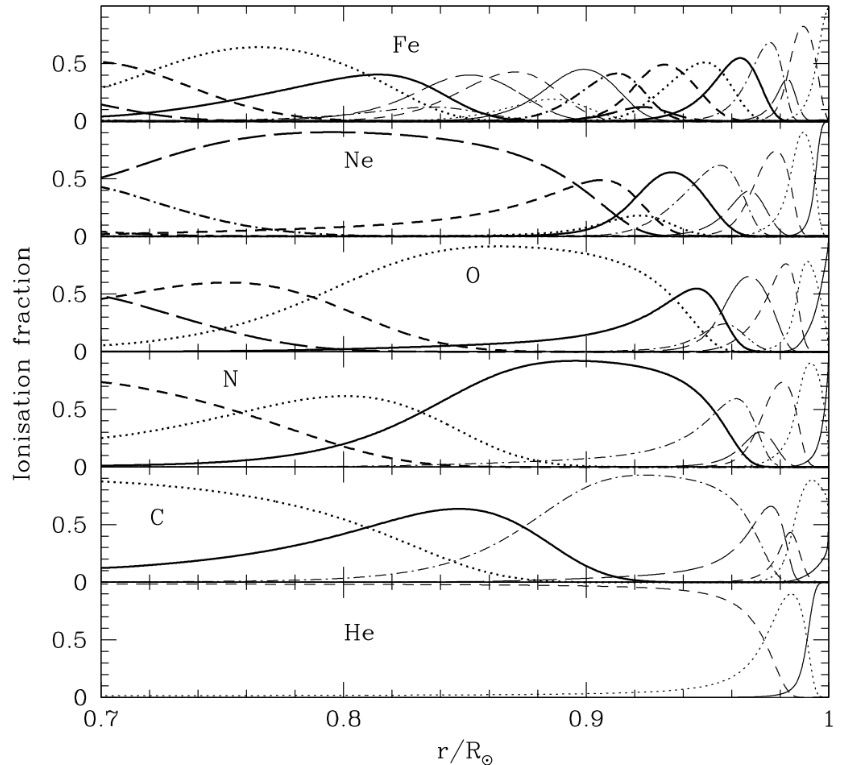
\includegraphics[width=0.4\textwidth,keepaspectratio]{ionfraction}\label{ionfraction}
       % \caption{Profilo radiale della popolazione dei diversi gradi di ionizzazione per $\cel{He}{4}{}{}$, CNO, $\cel{Ne}{20}{}{}$, $\cel{Fe}{56}{}{}$. Stati di ionizzazione maggiore sono pi\'u interni. Da \cite{basu2008helioseismology}.}
\end{figure}%

\end{itemize}

\end{frame}

\begin{frame}{Correzioni alla legge dei gas perfetti}



\end{frame}

\subsection{Tempo-scala dinamico}



\section{Trasporto dell'energia}

\section{Produzione di energia - reazioni di fusione}

\section{Modello solare standard e osservabili sismologiche}


